\documentclass[a4paper,12pt]{article}
\usepackage[ukrainian,english]{babel}
\usepackage{ucs}
\usepackage[utf8]{inputenc}
\usepackage[T2A]{fontenc}
\usepackage{amsmath}
\usepackage[export]{adjustbox}
\usepackage{amsfonts}
\usepackage{graphicx}
\usepackage{changepage}
\usepackage{multirow}
\usepackage{subcaption}
\usepackage{wrapfig}
\usepackage{array, makecell}
\usepackage[document]{ragged2e}
\usepackage{parskip}
\usepackage[paper=portrait,pagesize]{typearea}
\usepackage{multicol}
\newcommand\tab[1][1cm]{\hspace*{#1}}
\newcommand\dd{\textbf{ d}}
\newcommand\const{\textbf{const}}
\addto\captionsenglish{\renewcommand{\figurename}{Рис.}}
\addto\captionsenglish{\renewcommand{\tablename}{Таблиця}}
\usepackage{titlesec}
\usepackage[left=20mm, top=20mm, right=20mm, bottom=20mm, nohead, nofoot]{geometry}
%\titleformat{\section}[block]{\Large\bfseries\filcenter}{}{1em}{}
\titleformat{\subsection}[hang]{\bfseries}{}{1em}{}
\titleformat{\subsubsection}[hang]{\bfseries}{}{2em}{}
\begin{document}
	\begin{justify}
	\thispagestyle{empty}\setlength{\parindent}{0pt}
		\topskip0pt
	\vspace*{\fill}
		\begin{center}
			\LARGE{РОЗРАХУНКОВА РОБОТА З ЗАГАЛЬНОЇ ФІЗИКИ\\РОЗДІЛ "ЕЛЕКТРОДИНАМІКА"\\Варіант №2\\} 
			ФІ-12 Бекешева Анастасія 
		\end{center}
	\vspace*{\fill}\newpage
	\section{Умови}
	\begin{itemize}
		\item $\varepsilon=1$
		\item $\rho(r)=\rho_0\left(\dfrac{R_2}{r}\right)$
		\item $\rho_0=50\cdot10^{-9}\dfrac{\textrm{Кл}}{\textrm{м}^3}$
		\item $R_1=0.05\textrm{м}$
		\item $R_2=0.1\textrm{м}$
		\item $\sigma=0$
	\end{itemize}
	\section{Рисунок}
	\begin{figure}[!h]
    \centering
    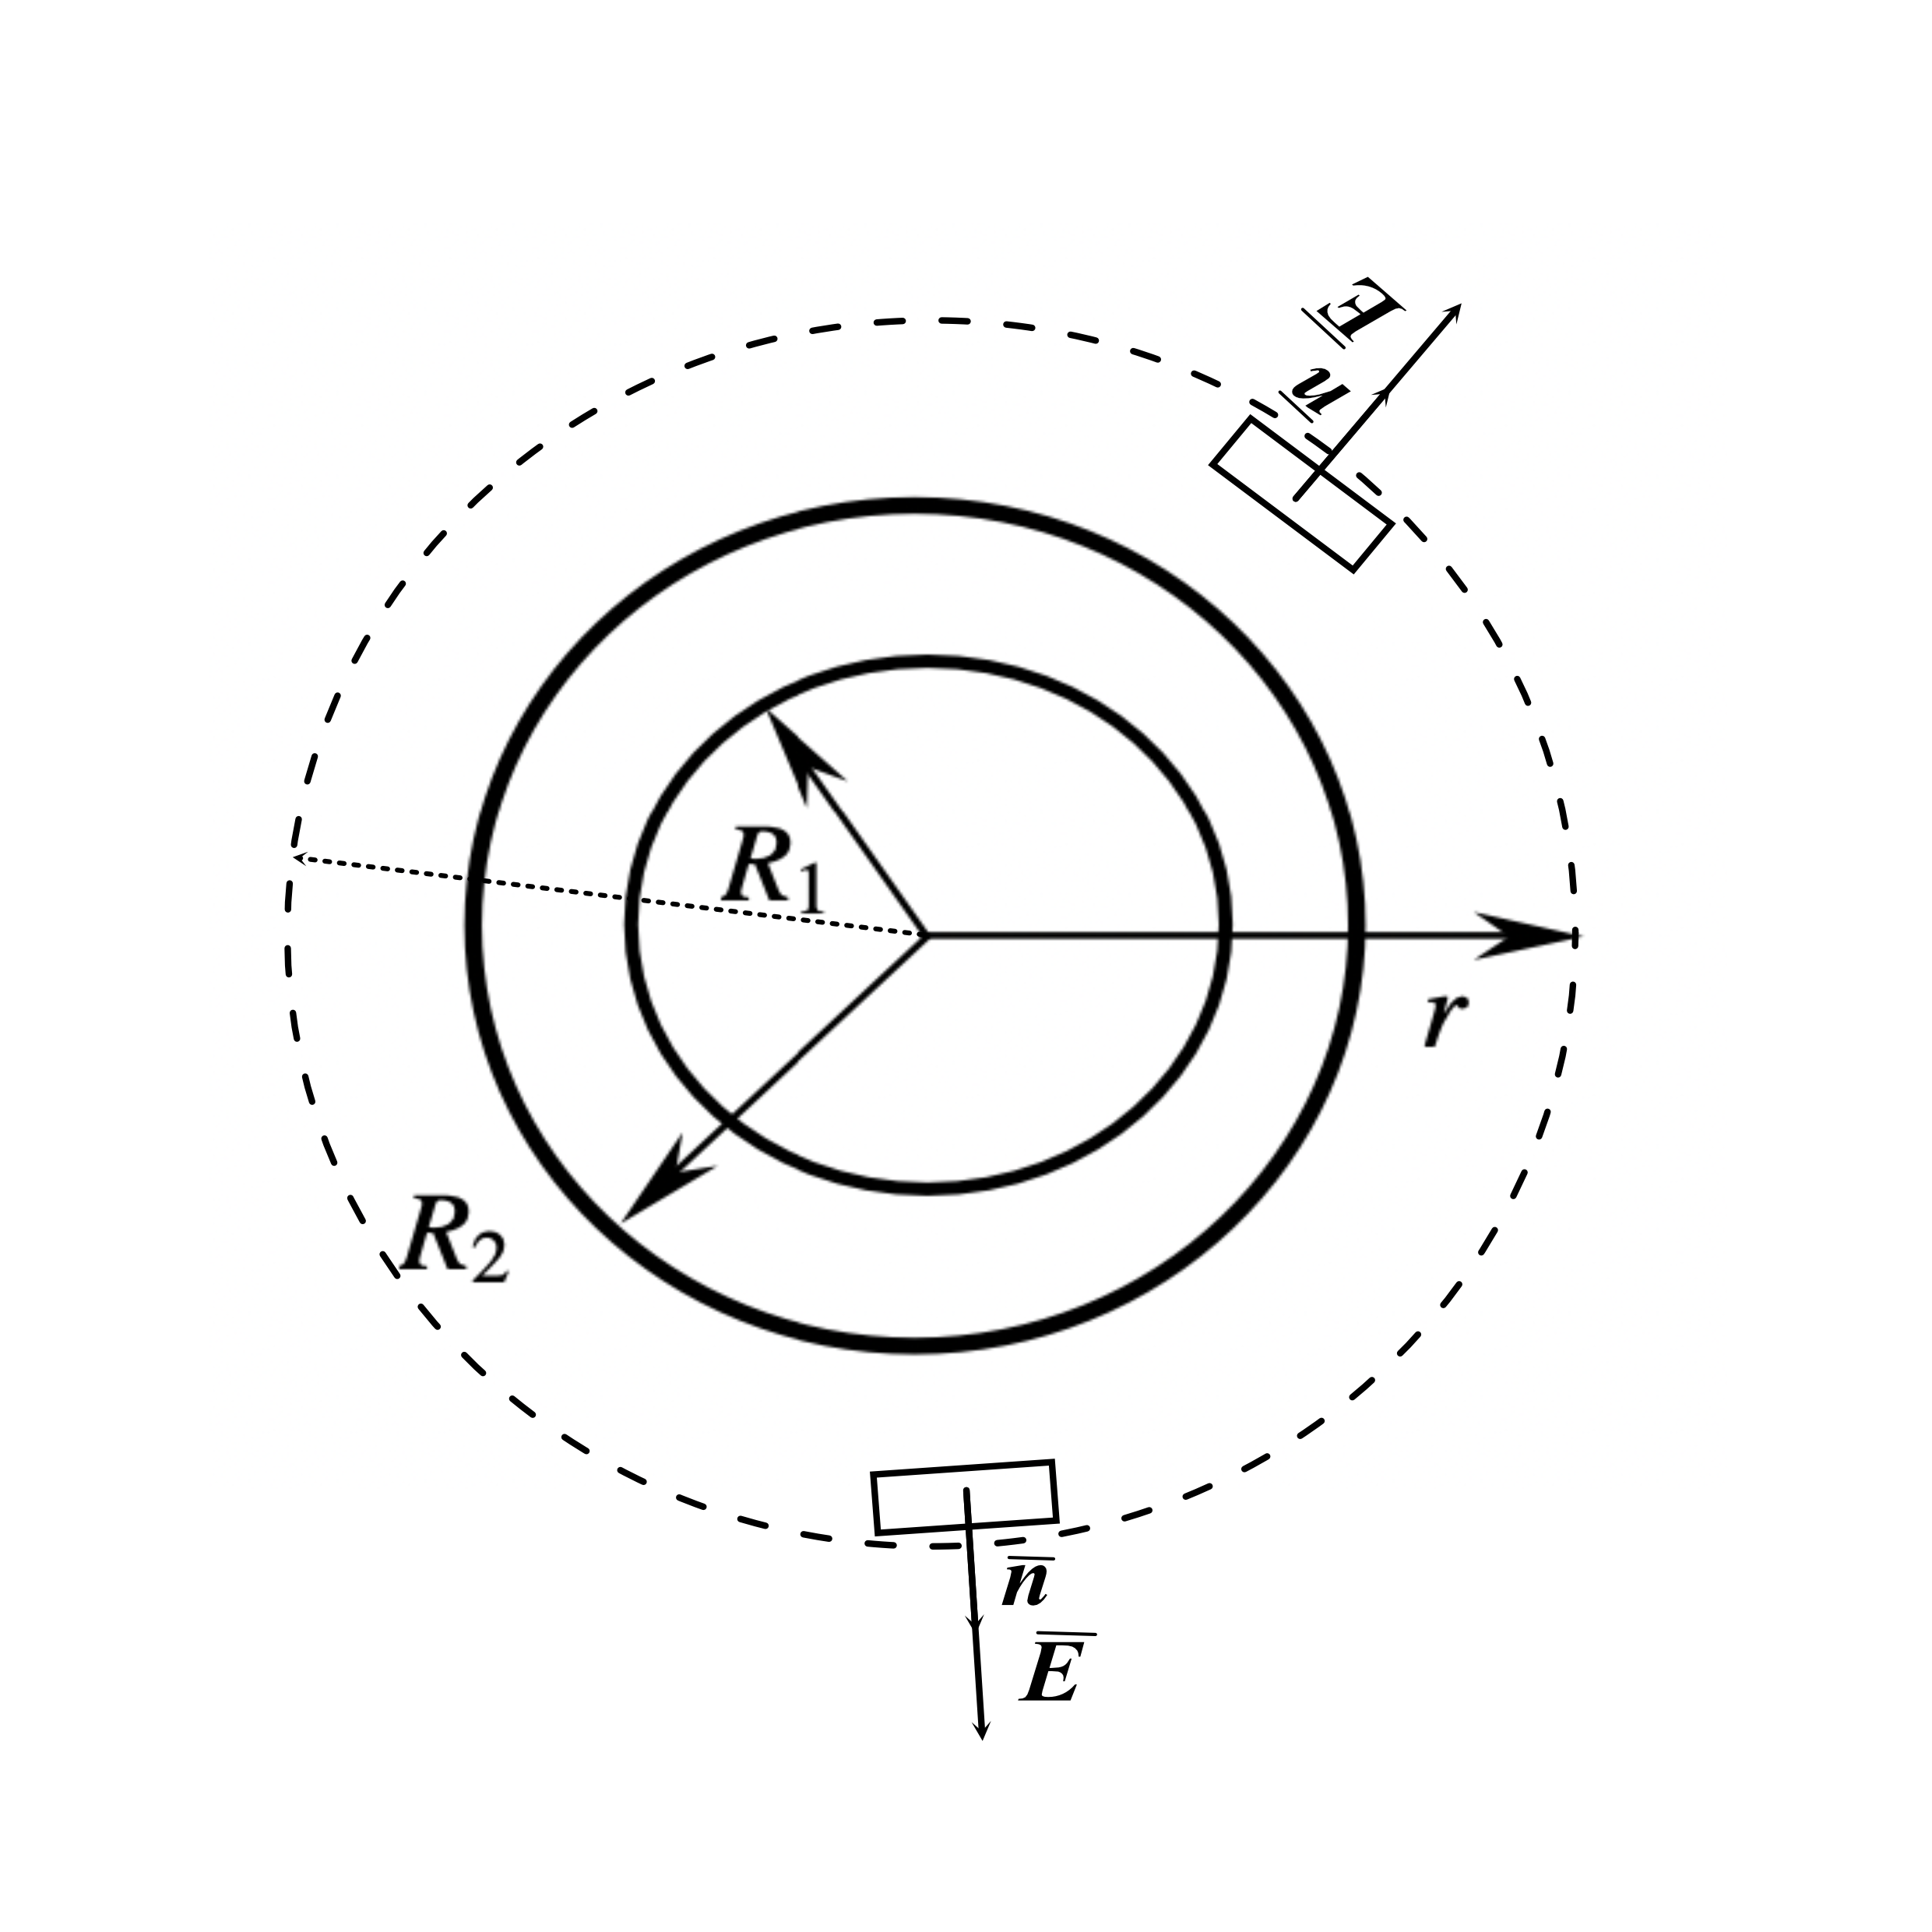
\includegraphics[width=10cm]{media/cw_graph1}
    \caption{Кульовий шар із зовнішнім та внутрішнім радіусами}
    \label{fig:1}
	\end{figure}
	\section{Вирази для $E_r(r)$}
	$\displaystyle\oint E\dd S=\dfrac{Q}{\varepsilon_0},\tab Q=\displaystyle\int\limits_{R_1}^{R_2}\rho\dd V+\sigma\cdot S$
	\subsection{$r<R_1$}
	Поле відсутнє. Зарядів у поверхні немає. $E=0$
	\begin{equation}
		E_1=0
	\end{equation}
	\subsection{$R_1\leq r\leq R_2$}
	$\rho=\dfrac{\dd Q_2}{\dd V},\tab \dd Q_2=\rho\cdot\dd V,\tab \dd V=S\dd r=4\bar{n}r^@\dd r,\tab Q_2=\displaystyle\int\rho\cdot S\dd r,\\Q_2=\displaystyle\int\limits_{R_1}^r\rho\cdot4\bar{n}r^2\dd r=\displaystyle\int\limits_{R_1}^r\rho_0\cdot4\bar{n}r^2\dfrac{R_2}{r}\dd r=\displaystyle\int\limits_{R_1}^r\rho_0\cdot4\bar{n}\cdot R_2\cdot r\dd r=\rho_0\cdot4\bar{n}\cdot R_2\displaystyle\int\limits_{R_1}^r r\dd r=\\=\rho_0\cdot4\bar{n}\cdot R_2\cdot\left.\dfrac{r^2}{2}\right|_{R_1}^r=2\rho_0\cdot\bar{n}\cdot R_2\\E=\dfrac{Q_2}{S\cdot\varepsilon_0}=\dfrac{2\rho_0\cdot\bar{n}\cdot R_2\cdot(r^2-R_1^2)}{4\bar{n}\cdot r^2\cdot\varepsilon_0}=\dfrac{\rho_0\cdot R_2\cdot(r^2-R^2_1)}{2r^2\cdot\varepsilon_0}$
	\begin{equation}
		E_2= \dfrac{\rho_0\cdot R_2\cdot(r^2-R^2_1)}{2r^2\cdot\varepsilon_0}
	\end{equation}
	\subsection{$r>R_2$}
	$Q_3=\displaystyle\int\rho\cdot D\dd r=\displaystyle\int\limits_{R_1}^{R_2}\rho_0\cdot4\bar{n}\cdot r^2\dfrac{R_2}{r}\dd r=\rho_0\cdot 4\bar{n}\cdot R_2\left.\dfrac{r^2}{2}\right|_{R_1}^{R_2}=2\rho_0\cdot\bar{n}\cdot R_2\cdot(R_1^2-R_2^2)\\E=\dfrac{Q_3}{S\cdot\varepsilon_0}=\dfrac{2\rho_0\cdot\bar{n}\cdot R_2\cdot(R_2^2-R_1^2)}{4\bar{n}\cdot r^2\cdot\varepsilon_0}=\dfrac{\rho_0\cdot R_2\cdot(R_2^2-R_1^2)}{2r^2\cdot\varepsilon_0}$
	\begin{equation}
		E_3=\dfrac{\rho_0\cdot R_2\cdot(R_2^2-R_1^2)}{2r^2\cdot\varepsilon_0}
	\end{equation}
	\section{Вирази для $\varphi(r)$}
	\subsection{$r<R_1$}
	$\varphi=\const=0$
	\begin{equation}
		\varphi_1=0
	\end{equation}
	\subsection{$R_1\leq r\leq R_2$}
	$\varphi=\displaystyle\int E\dd r=\displaystyle\int\dfrac{\rho_0\cdot R_2\cdot(r^2-R^2_1)}{2r^2\cdot\varepsilon_0}\dd r=\dfrac{\rho_0R_2}{2\varepsilon_0}\displaystyle\int\dfrac{r^2-R_1^2}{r^2}\dd r=-\dfrac{\rho_0R_2}{2\varepsilon_0}\left(\dfrac{r^2-R_1^2}{r}+2r\right)+c$
	\begin{equation}
		\varphi_2=c\dfrac{\rho_0\cdot R_2}{2\varepsilon_0}\left(\dfrac{3r^2-R_1^2}{r}\right)+c
	\end{equation}
	\subsection{$r>R_2$}
	$\varphi=\displaystyle\int E\dd r=\displaystyle\int\dfrac{\rho_0\cdot R_2\cdot(R_2^2-R_1^2)}{2r^2\cdot\varepsilon_0}\dd r=\dfrac{\rho_0R_2(R_2^2-R_1^2)}{2\varepsilon_0}\displaystyle\int\dfrac{\dd t}{r^2}=-\dfrac{\rho_0\cdot R_2\cdot(R_2^2-R_1^2)}{2\varepsilon_0}\cdot\dfrac{1}{r}+c$
	\begin{equation}
		\varphi_3=-\dfrac{\rho_0\cdot R_2\cdot(R_2^2-R_1^2)}{2\varepsilon_0}\cdot\dfrac{1}{r}+c
	\end{equation}
	\section{Числові формули}
	$\varphi_2=\varphi_3\tab\Rightarrow\tab -\dfrac{\rho_0\cdot R_2}{2\varepsilon_0}\left(\dfrac{3r^2-R_1^2}{r}\right)+c=-\dfrac{\rho_0\cdot R_2\cdot(R_2^2-R_1^2)}{2\varepsilon_0}\cdot\dfrac{1}{r}\\\dfrac{3r^2-R_1^2}{r}+c=\dfrac{R_2^2-R_1^2}{r},\tab c=\dfrac{R_2^2-3r^2}{r}=\dfrac{R_2^2-3R_2^2}{R^2}=-2R_2=-2\cdot0.1=-0.2$
	\begin{equation}
		\varphi_2=-\dfrac{\rho_0\cdot R_2}{2\varepsilon_0}\left(\dfrac{3r^2-R_1^2}{r}\right)-0.2\textrm{ Н}\cdot\dfrac{\textrm{Кл}^2}{\textrm{м}}
	\end{equation}
	\begin{equation}
		\varphi_2=-\dfrac{\rho_0\cdot R_2\cdot(R_2^2-R_1^2)}{2\varepsilon_0}\cdot\dfrac{1}{r}-0.2\textrm{ Н}\cdot\dfrac{\textrm{Кл}^2}{\textrm{м}}
	\end{equation}
	\section{Розрахунок}
	
	
	
	
	
	
	
	
	
	
	
	
	
	
	
	
	
	
	
	
	
	
	
	
	
	
	
	
	
	
	
	\end{justify}
\end{document}